% =====================================================================
%  Online controller selection for the angular control of
%  gravitational-wave detectors under non-stationary noise
%
%  FIRST DRAFT.  Sections marked with \todo{...} are placeholders or
%  require results not yet produced (notably the bandit experiments).
%  Compile with pdflatex (standard packages only; no bibtex needed).
% =====================================================================
\documentclass[11pt,a4paper]{article}

\usepackage[utf8]{inputenc}
\usepackage[T1]{fontenc}
\usepackage{amsmath,amssymb}
\usepackage{graphicx}
\usepackage{booktabs}
\usepackage{xcolor}
\usepackage[margin=2.5cm]{geometry}
\usepackage[colorlinks=true,linkcolor=blue,citecolor=blue,urlcolor=blue]{hyperref}
\usepackage{authblk}

\emergencystretch=2em % prefer stretched spaces over margin overflow

% Lightweight unit macro (avoids the siunitx dependency); works in math and text.
\newcommand{\SI}[2]{#1\,\text{#2}}
\newcommand{\si}[1]{\text{#1}}
\newcommand{\todo}[1]{\textcolor{red}{\textbf{[TODO: #1]}}}
\newcommand{\Chard}{u_{\mathrm{h}}}
\newcommand{\ehard}{e_{\mathrm{h}}}
\newcommand{\Cz}{C_{0}}
\newcommand{\Co}{C_{1}}
\newcommand{\Ct}{C_{2}}

\title{\bfseries Online controller selection for the angular control of
gravitational-wave detectors under non-stationary noise:\\
a multi-armed bandit approach}

\author[1]{Marco Grillo}
\author[1,2]{Tomislav Andric}
\author[1,2]{Jan Harms}
\affil[1]{Gran Sasso Science Institute (GSSI), I-67100 L'Aquila, Italy}
\affil[2]{INFN, Laboratori Nazionali del Gran Sasso, I-67100 Assergi, Italy}

\date{Draft --- \today}

\begin{document}
\maketitle

\begin{abstract}
The angular control loops of gravitational-wave (GW) detectors must reject
radiation-pressure (Sidles--Sigg) torques whose strength, together with the
seismic and sensing-noise environment, varies over time. In current operation
the choice of control filter is changed by hand by operators, for instance
switching from low- to high-gain alignment control when an earthquake
early-warning system forecasts elevated ground motion. We formulate this
choice as an \emph{online controller-selection} problem and study whether a
multi-armed bandit policy can perform the selection autonomously so as to
minimise a long-horizon cost. Using a time-domain simulator of the pitch
degree of freedom of a coupled-cavity detector, validated against a reference
implementation, we define three operating regimes and a family of fixed linear
controllers with a designed one-to-one regime--controller correspondence, and
a scalar reward built from the hard-eigenmode error and control effort. We make
three contributions ahead of the bandit study itself. First, we characterise
the reward landscape and show that the designed one-to-one regime--controller
mapping holds in all three regimes, robustly in the nominal and intermediate
regimes and marginally in the extreme regime, with a non-saturating reward.
Second, we
quantify the cost of switching controllers and find a pronounced asymmetry:
gain-decreasing switches are far costlier than gain-increasing ones. Third, and
most importantly, we show that the apparent switching penalty is dominated by
the \emph{controller-handover implementation}: a naive state reset or raw
state carry-over produces large transients, whereas a bumpless, parallel-bank
handover renders the switching cost negligible for this gain-scaled controller
family. Finally, we introduce \emph{Recurrence-Aware Thompson Sampling}
(RA-TS-F), a minimal policy combining Thompson sampling with a drift detector, a
library of per-regime posteriors that are \emph{resumed} when a regime recurs,
and a bounded coverage probe. On one-week and six-month simulated benchmarks
RA-TS-F attains the lowest regret of all policies tested---non-stationary
bandit baselines, an operator-like rule-based policy, and every fixed
controller---capturing $74$--$83\%$ of the oracle's achievable advantage over
the best fixed controller, with a regret $4$--$7\times$ lower than every
alternative over six months.
\end{abstract}

% =====================================================================
\section{Introduction}\label{sec:intro}
% ---------------------------------------------------------------------
Second-generation gravitational-wave detectors such as Advanced
LIGO~\cite{aLIGO} and Advanced Virgo~\cite{aVirgo} are kilometre-scale
Fabry--Perot--Michelson interferometers whose test masses are suspended as
multi-stage pendula. Beyond the longitudinal degrees of freedom used to read out
the GW signal, the \emph{angular} degrees of freedom of the mirrors must be
actively controlled: residual angular motion couples to the longitudinal
signal and, more fundamentally, the circulating optical power exerts
radiation-pressure torques that soften one angular eigenmode and stiffen the
other---the Sidles--Sigg effect~\cite{SidlesSigg}. The alignment sensing and
control (ASC) loops that stabilise these modes operate close to a
power-dependent instability and are a recognised limit to detector duty cycle
and low-frequency sensitivity~\cite{Barsotti}.

The disturbance environment of these loops is strongly non-stationary. Ground
motion exhibits a diurnal cycle, a microseismic band that is modulated by
weather and oceanic activity on timescales of hours to days, and rare, intense
transients associated with earthquakes and storms. A single fixed controller
cannot be simultaneously optimal across this range of conditions: a high-gain
loop that rejects large low-frequency disturbances injects excess control
noise when the environment is quiet, while a low-gain loop that is quiet in
nominal conditions fails to maintain alignment during elevated ground motion.
In current practice this trade-off is managed manually: operators (or simple
rule-based logic) switch between predefined control filters, for example moving
to a high-gain alignment configuration when an earthquake early-warning system
predicts high incoming ground motion.

This manual, forecast-driven switching is a natural candidate for automation. We
pose it as an \emph{online controller-selection} problem: given a fixed library
of controllers and a scalar performance signal computed online from the loop's
own error and control signals, an autonomous policy must repeatedly choose which
controller to apply so as to minimise the time-integrated cost, without prior
knowledge of when the environment will change. This is precisely the setting of
the \emph{non-stationary multi-armed bandit}~\cite{Lattimore,GarivierMoulines,
AdSwitch}: each controller is an arm, the negative cost is a stochastic reward
whose distribution shifts when the environment changes, and the policy must
balance exploration (testing controllers to detect such shifts) against
exploitation (using the controller currently believed best).

In this work we build the simulation and problem infrastructure required to
study this question rigorously, and we report a set of results that are
prerequisites to---and partly independent of---the choice of bandit algorithm.
Our contributions are:
\begin{enumerate}
  \item A time-domain detector model with an explicit, validated plant, in which
  three operating regimes and a family of fixed linear controllers are defined
  so as to admit a designed one-to-one regime--controller mapping
  (Sections~\ref{sec:framework}--\ref{sec:problem}).
  \item A characterisation of the resulting reward landscape
  (Section~\ref{sec:reward}), establishing that the one-to-one mapping holds in
  all three regimes (robustly in the nominal and intermediate regimes, marginally
  in the extreme regime) and that the reward is non-saturating, so a learnable
  signal is present in every regime.
  \item A quantitative study of the \emph{dynamics of switching}
  (Section~\ref{sec:switch}): the transient cost of changing controllers, its
  asymmetry in the direction of the gain change, and---central to the
  feasibility of online switching---the dependence of this cost on the
  controller-handover implementation, with the conclusion that a realistic
  bumpless handover makes switching nearly free.
  \item An online-selection policy, \emph{Recurrence-Aware Thompson Sampling
  with a coverage floor} (RA-TS-F), designed around the structure established in
  1--3: regimes recur, their identity is carried by the \emph{shape} of the
  per-arm rewards rather than their level, and switching is cheap. On one-week
  and six-month benchmarks with a common noise realisation across policies,
  RA-TS-F attains the lowest regret of every policy tested
  (Section~\ref{sec:bandit}).
\end{enumerate}

% =====================================================================
\section{Background}\label{sec:background}
% ---------------------------------------------------------------------
\subsection{Angular control and the Sidles--Sigg effect}\label{sec:bg-ss}
Consider the two test masses forming a single arm cavity of length $L$ with
radii of curvature $R_1$ (input, ITM) and $R_2$ (end, ETM). In the pitch
(vertical-plane tilt) degree of freedom, the cavity geometry is described by the
$g$-factors $g_i = 1 - L/R_i$. The radiation pressure of the circulating power
couples the two mirror tilts; diagonalising the coupling yields two angular
eigenmodes, conventionally termed \emph{soft} and \emph{hard}, with
optical-spring-modified torsional stiffnesses. The transformation from the local
(ITM, ETM) tilt basis to the eigenbasis is
\begin{equation}
  r = \tfrac{1}{2}\!\left(g_1 - g_2 + \sqrt{(g_1-g_2)^2 + 4}\right),\qquad
  T_{\mathrm{loc}\to\mathrm{eig}} = \frac{1}{1+r^2}\begin{pmatrix} 1 & r \\ -r & 1\end{pmatrix},
  \label{eq:eigen}
\end{equation}
and the beam-spot-to-angle response factors of the two modes are
\begin{equation}
  \frac{\partial y}{\partial\theta}\bigg|_{\mathrm{soft/hard}}
  = \frac{L}{2}\,\frac{(g_1+g_2)\pm\sqrt{(g_2-g_1)^2+4}}{g_1 g_2 - 1}.
  \label{eq:dydth}
\end{equation}
For the parameters of interest the hard mode is the limiting loop: it carries
the dominant radiation-pressure torque and is the relevant control-noise
injection path, and we therefore use it as the sole performance channel
throughout (Section~\ref{sec:problem}). The circulating power that sets the
strength of this coupling follows the Fabry--Perot resonance condition
\begin{equation}
  P_{\mathrm{cav}} = \frac{P_{\mathrm{in}}\,T_1}
  {\left|\,1 - \sqrt{R_1 R_2}\,\exp\!\big(4\pi i\,\delta L_{\mathrm{hp}}/\lambda\big)\right|^2},
  \label{eq:cavpow}
\end{equation}
with $T_1$ the ITM power transmissivity, $\lambda$ the laser wavelength, and
$\delta L_{\mathrm{hp}}$ the high-passed cavity-length change induced by the
mirror tilts.

\subsection{The non-stationary disturbance environment}\label{sec:bg-env}
The seismic input to the suspensions varies on multiple timescales: a diurnal
component, a microseismic band modulated by weather over hours to days, and
sporadic high-amplitude transients. Operationally, this motivates a small set of
qualitatively distinct \emph{regimes} and a corresponding set of controllers
tuned for each, between which the configuration is switched. A key methodological
point, which we adopt throughout, is that physically relevant non-stationarity
is \emph{adiabatic}: the environment evolves continuously rather than by abrupt
steps, so that the interesting question is whether control remains stable, and a
selection policy beneficial, \emph{through} the slow transitions
\cite{Harms_internal}. \todo{cite the LIGO/MIT operational practice of
earthquake-triggered low/high-gain ASC switching with a proper reference.}

\subsection{Bandits for non-stationary rewards}\label{sec:bg-bandit}
In the stochastic multi-armed bandit, a policy repeatedly selects one of $K$
arms and observes a reward drawn from that arm's (unknown) distribution, with
the goal of minimising regret relative to the best arm~\cite{Lattimore}. When
the reward distributions change over time the relevant notion is
\emph{non-stationary} regret against the best arm \emph{at each time}. Two broad
families address this: passively forgetting methods, such as discounted or
sliding-window UCB~\cite{GarivierMoulines} and exponential-weighting variants;
and actively adaptive methods that detect distribution changes, of which
AdSwitch~\cite{AdSwitch} is a representative with regret guarantees under an
unknown number of changes. Under milder, more informative statistical
assumptions about the regimes, Bayesian approaches such as Thompson
sampling~\cite{Thompson,RussoTutorial}, possibly in a contextual form, may
exploit structure that the worst-case methods cannot. The appropriate choice
depends on the regime-switching statistics and the separation of the per-arm
reward distributions; quantifying the latter is one purpose of
Section~\ref{sec:reward}. A third structural feature, central to our setting,
is \emph{recurrence}: the environment does not drift to ever-new states but
revisits a small set of regimes. A policy that re-learns each regime from
scratch on every visit pays the identification cost repeatedly; a policy that
recognises a returning regime and resumes previously accumulated knowledge pays
it once. Exploiting recurrence, with change detection in the spirit of
CUSUM-type tests~\cite{Page}, is the design principle behind the policy of
Section~\ref{sec:ba-rats}.

% =====================================================================
\section{Simulation framework}\label{sec:framework}
% ---------------------------------------------------------------------
\subsection{Time-domain plant model}\label{sec:fw-plant}
We use a time-domain simulator (``Lightsaber'') of the pitch degree of freedom
of a single arm cavity, run as a per-sample closed loop at a sampling frequency
$f_s = \SI{256}{Hz}$. The principal parameters are an arm length
$L = \SI{3994.5}{m}$, radii of curvature $R_1 = \SI{1934}{m}$ and
$R_2 = \SI{2245}{m}$, ITM transmissivity $T_1 = 0.014$, laser wavelength
$\lambda = \SI{1064}{nm}$, and a nominal arm-cavity input power
$P_{\mathrm{in}} = \SI{705}{W}$ (corresponding to a nominal circulating power of
order \SI{200}{kW}).

At each time step the plant (i) injects test-mass pitch noise obtained by
filtering colored seismic and damping-loop (OSEM) noise through measured
suspension transfer functions; (ii) computes the cavity power from
Eq.~\eqref{eq:cavpow}; (iii) forms the radiation-pressure torques on the two
masses,
\begin{equation}
  \tau = \frac{2}{c}\Big(P_{\mathrm{cav}}\,\mathbf{s} + \mathbf{s}_0\,(P_{\mathrm{cav}}-P_{\mathrm{dc}})\Big),
  \label{eq:torque}
\end{equation}
with $\mathbf{s}$ the beam-spot vector, $\mathbf{s}_0$ a static beam-spot offset
defining the operating point, and $P_{\mathrm{dc}}$ a reference power; (iv)
propagates torque and actuation to mirror angle through the radiation-pressure
($\mathrm{TM}{\to}\mathrm{P}$) and actuator ($\mathrm{PUM}{\to}\mathrm{TM}$)
state-space models; (v) reads out the two eigenmodes via
Eq.~\eqref{eq:eigen} with additive sensing noise; (vi) applies a
power-dependent Sidles--Sigg compensation path; and (vii) computes the
controller actuation. The controllers act on the eigenmode error and their
output is mapped back to the local actuation basis. All recursive elements
(plant, compensator, controller) are second-order-section (SOS) digital filters
with persistent internal state, so that the simulation is a faithful continuous
closed loop rather than a sequence of independent batches.

\subsection{Validation against the reference simulator}\label{sec:fw-valid}
The plant used here is a refactored version of an earlier, component-graph
reference implementation. We verified that the refactoring preserves the
physics. The two core plant transfer functions---the actuator response
($\mathrm{PUM}{\to}\mathrm{TM}$, gain $93.53$) and the radiation-pressure
response ($\mathrm{TM}{\to}\mathrm{P}$, gain $2.5677$)---are identical
zero--pole--gain models; the three measured suspension transfer functions are
bit-identical between the two codebases (maximum amplitude difference $0$); and
the high-pass, Fabry--Perot, eigenmode and beam-spot expressions coincide. The
differences between the two implementations are confined to the deliberately
modified experimental layer---the static operating point $\mathbf{s}_0$, the
form of the Sidles--Sigg compensator, the controller family
(Section~\ref{sec:problem}), and the regime-dependent noise inputs---and none
constitutes a change to the underlying plant. We therefore treat the present
plant as physically equivalent to the reference. \todo{Optionally add a
quantitative dynamic cross-check (matched-configuration output PSD overlay).}

% =====================================================================
\section{Problem formulation}\label{sec:problem}
% ---------------------------------------------------------------------
\subsection{Operating regimes}\label{sec:pr-regimes}
We define three operating regimes that differ along physically motivated axes:
the optical power (and hence the Sidles--Sigg coupling strength), the seismic
input level, and the sensing (readout) noise. The scale factors, applied to the
nominal configuration, are listed in Table~\ref{tab:regimes}; the underlying
amplitude spectral densities are derived from O4-era data. Regime $R_0$ is the
nominal, low-ground-motion state; $R_1$ a high-microseism state; and $R_2$ an
extreme state with strongly elevated seismic input but a comparatively clean
sensor.

\begin{table}[t]
  \centering
  \caption{Regime definitions: multiplicative scale factors applied to the
  nominal configuration.}
  \label{tab:regimes}
  \begin{tabular}{lccc}
    \toprule
     & $R_0$ (nominal) & $R_1$ (high-micro) & $R_2$ (extreme) \\
    \midrule
    Optical-power scale          & 1.00 & 0.95 & 0.90 \\
    Sensing-noise scale          & 120  & 12   & 0.25 \\
    Seismic-input scale          & 1.0  & 6.0  & 20.0 \\
    OSEM (damping) scale         & 1.0  & 1.0  & 1.0  \\
    \bottomrule
  \end{tabular}
\end{table}

\subsection{Controller family}\label{sec:pr-ctrl}
We consider three fixed hard-mode controllers, $\Cz$, $\Co$, $\Ct$, which share
an identical filter shape and differ only by an overall DC gain
($30$, $44.2$, $50$ respectively). They are therefore a one-parameter gain
family: driven by the same error signal, their outputs are proportional,
$u^{(j)} = (g_j/g_i)\,u^{(i)}$. The goal is to \emph{select} among them online,
not to retune them. The soft-mode controller is common to all three and is not
varied.

\subsection{Observables and scalar reward}\label{sec:pr-reward}
Performance is assessed on the hard eigenmode only, through two observables: the
hard-mode error signal $\ehard$ (the controller input/readout) and the hard-mode
control effort $\Chard$ (the controller output, transformed to the eigenbasis).
A linear scalarisation of error and control, $J = \alpha\,\mathrm{RMS}(\ehard) +
\beta\,\mathrm{RMS}(\Chard)$, cannot yield a consistent regime--controller
preference, because different regimes call for opposite error/control
trade-offs; a fixed trade-off slope therefore fails. We instead use a
multiplicative (logarithmic) cost. In its minimal form,
\begin{equation}
  J = \rho\,\log\!\frac{\mathrm{RMS}(\ehard)}{\min_C \mathrm{RMS}(\ehard)}
    + \log\!\frac{\mathrm{RMS}_{10\text{--}30\,\mathrm{Hz}}(\Chard)}
                 {\min_C \mathrm{RMS}_{10\text{--}30\,\mathrm{Hz}}(\Chard)},
  \label{eq:logcost}
\end{equation}
with a single global coefficient $\rho \approx 1.095$, which already yields the
intended one-to-one mapping. In the implementation used for the bandit reward we
adopt a generalised, multi-band form: the error and control signals are
decomposed into a set of Butterworth frequency bands, and the reward is a
weighted sum of the log band-powers evaluated on \SI{2}{s} blocks,
\begin{equation}
  Z = \sum_i w_i \log b_i, \qquad r_{\mathrm{raw}} = -Z,
  \label{eq:zreward}
\end{equation}
with band features $b_i$ (RMS per band of $\ehard$ and $\Chard$) and fixed
weights $w_i$ calibrated so as to reproduce the designed mapping. Because the
downstream policy expects a bounded reward, the per-segment mean raw score is
mapped to $[0,1]$ by a logistic,
\begin{equation}
  r = \big[\,1 + \exp\!\big(-(\bar r_{\mathrm{raw}} - r_0)/\sigma_0\big)\big]^{-1},
  \qquad r_0 = 167.5,\ \sigma_0 = 2.5.
  \label{eq:logistic}
\end{equation}
The implications of this normalisation are examined in
Section~\ref{sec:reward}.

\subsection{Designed regime--controller mapping}\label{sec:pr-map}
The regimes and controllers are constructed so that, under the cost of
Eq.~\eqref{eq:logcost}--\eqref{eq:zreward}, each regime has a distinct optimal
controller: $R_0 \to \Cz$, $R_1 \to \Co$, $R_2 \to \Ct$. Physically, the noisy
sensor of $R_0$ favours the low-gain controller (which injects less control
noise), while the clean sensor and elevated seismic input of $R_2$ favour the
high-gain controller (which rejects the larger disturbance). The accuracy of
this mapping is the subject of Section~\ref{sec:reward}.

% =====================================================================
\section{Characterisation of the reward landscape}\label{sec:reward}
% ---------------------------------------------------------------------
We characterise the reward of every controller in every regime by simulating
all nine (regime, controller) combinations. The band features are obtained by
filtering each error/control signal \emph{continuously} (the band-pass filter
state is carried across the run; the lowest band, $0.05$--$0.3$\,Hz, carries the
largest weight and requires this), and the reward of Eq.~\eqref{eq:zreward} is
the mean over \SI{2}{s} blocks. Statistics are accumulated over five independent
noise realisations (seeds) of \SI{360}{s} each; discarding a \SI{60}{s} filter
warm-up per realisation leaves $149$ settled \SI{2}{s} blocks per seed, $745$
pooled per cell in total. This pooled set of $745$ per-cell blocks is what the
histograms of Fig.~\ref{fig:reward} (top) show. Because the $149$ blocks within
one realisation come from a continuously-stateful filter, consecutive blocks
are autocorrelated and cannot be treated as independent draws for an error
estimate; we therefore first average the $149$ blocks of each realisation down
to a single per-seed mean reward, and report the bar heights and error bars of
Fig.~\ref{fig:reward} (bottom) as the mean and standard error \emph{of those
five per-seed means} (five genuinely independent samples), not of the $745$
raw blocks. Table~\ref{tab:reward} reports the corresponding mean raw and
logistic-mapped reward.

\begin{table}[t]
  \centering
  \caption{Mean reward per (regime, controller). Raw score $r_{\mathrm{raw}}$
  [Eq.~\eqref{eq:zreward}] and logistic (bandit-space) reward
  [Eq.~\eqref{eq:logistic}]. Bold marks the per-regime optimum.}
  \label{tab:reward}
  \begin{tabular}{l ccc c ccc}
    \toprule
     & \multicolumn{3}{c}{raw $r_{\mathrm{raw}}$} & & \multicolumn{3}{c}{logistic $r$} \\
     \cmidrule(lr){2-4}\cmidrule(lr){6-8}
     & $\Cz$ & $\Co$ & $\Ct$ & & $\Cz$ & $\Co$ & $\Ct$ \\
    \midrule
    $R_0$ & \textbf{168.59} & 167.75 & 167.38 & & \textbf{0.597} & 0.521 & 0.487 \\
    $R_1$ & 165.52 & \textbf{165.68} & 165.39 & & 0.325 & \textbf{0.338} & 0.314 \\
    $R_2$ & 167.43 & 168.23 & \textbf{168.28} & & 0.492 & 0.565 & \textbf{0.569} \\
    \bottomrule
  \end{tabular}
\end{table}

\begin{figure}[t]
  \centering
  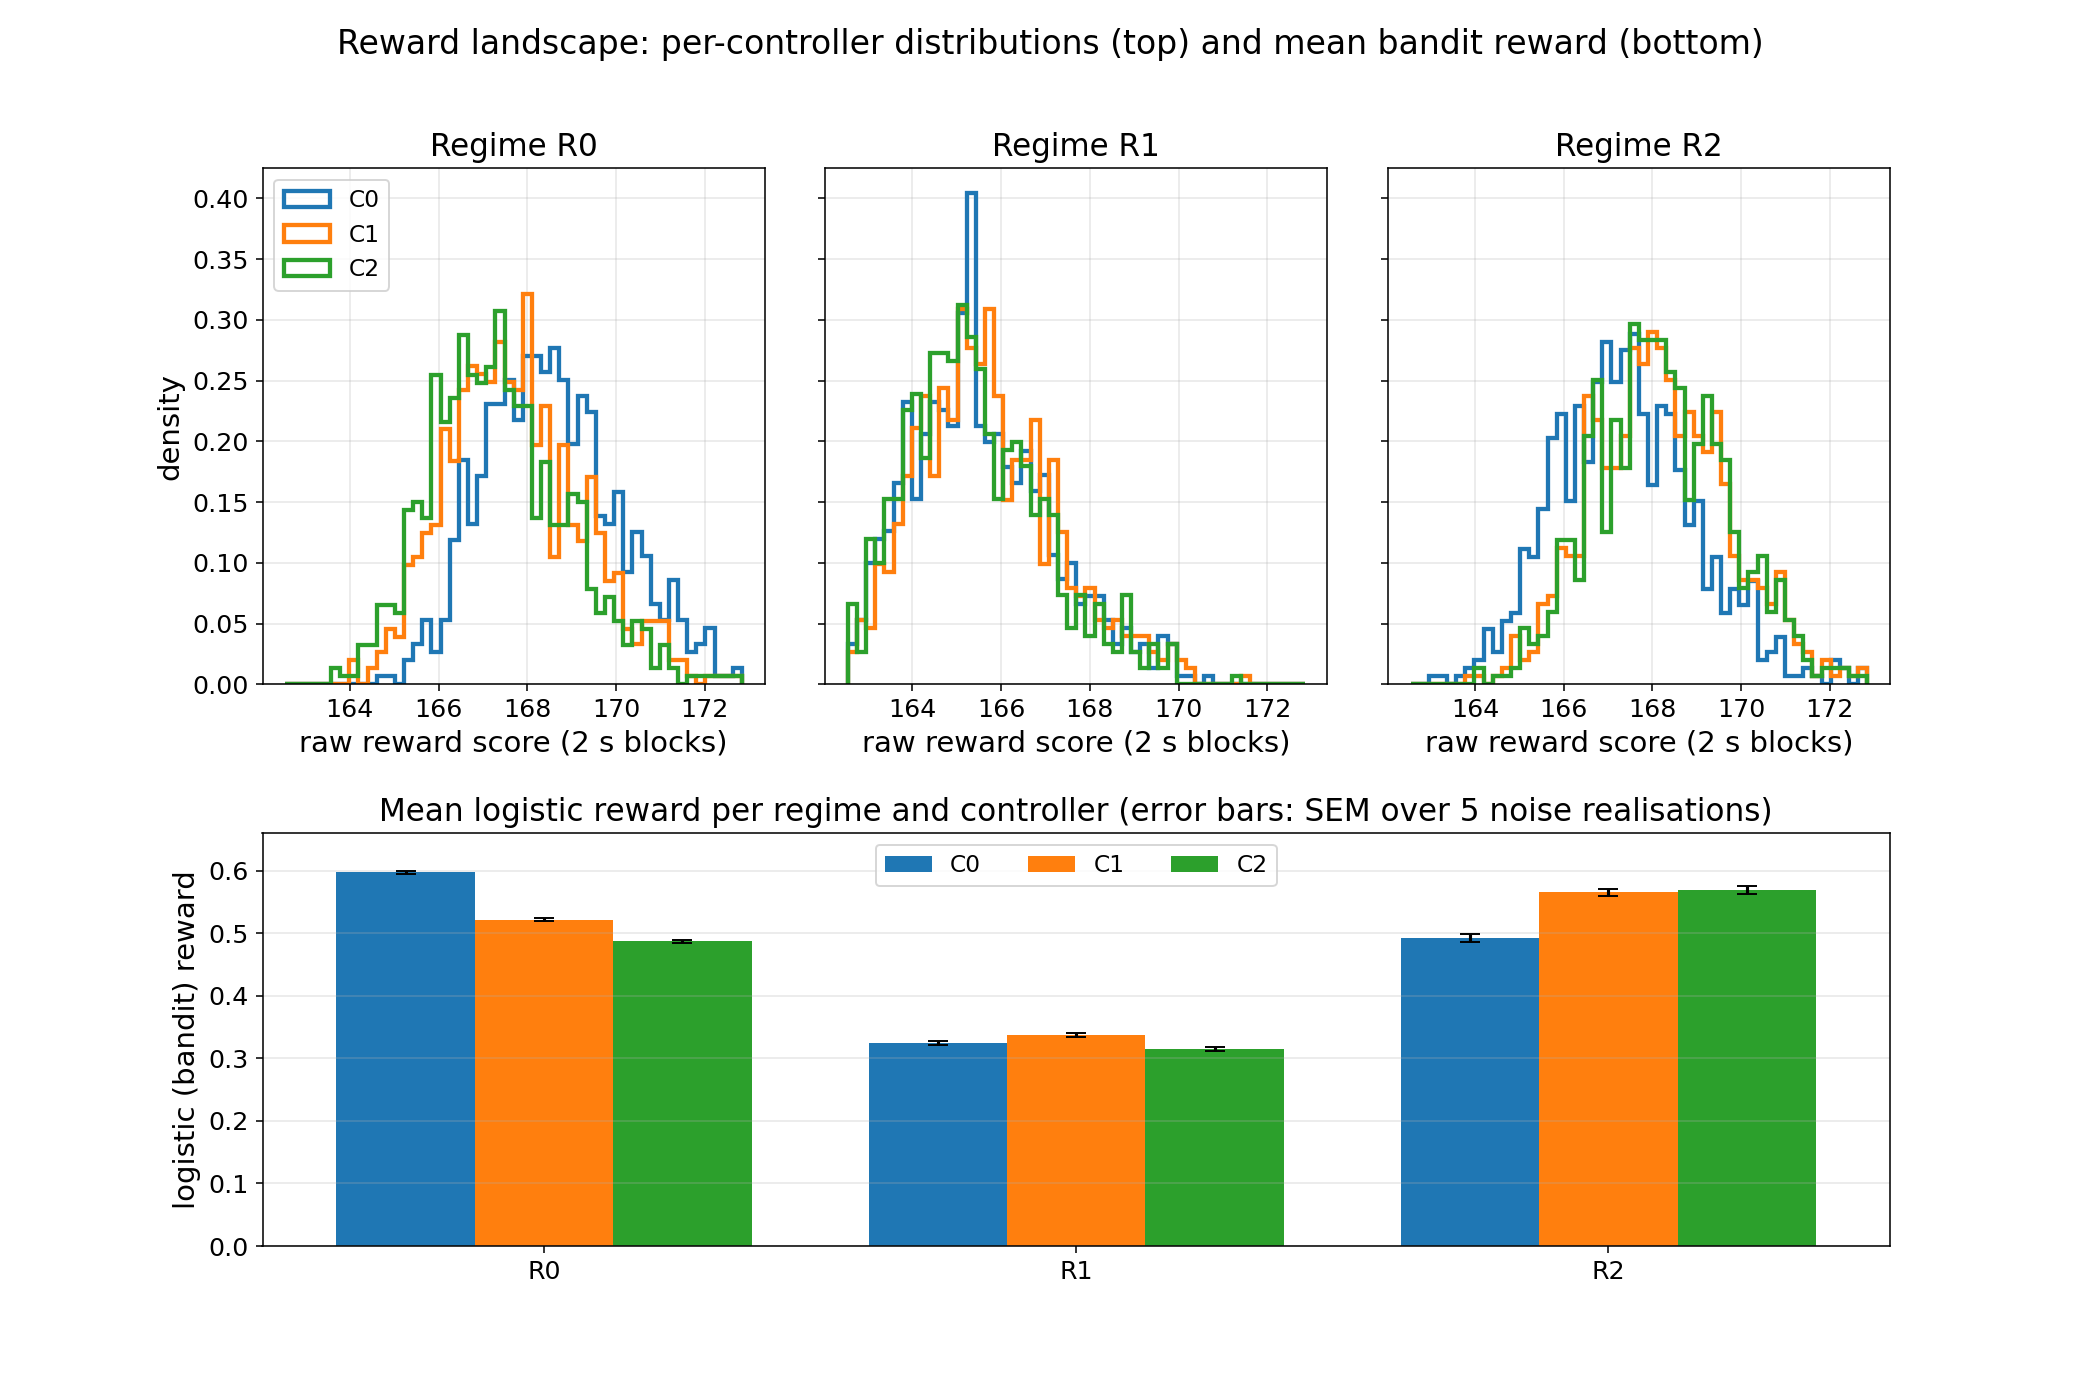
\includegraphics[width=\linewidth]{figs/reward_landscape.png}
  \caption{Reward landscape: the same data at two levels of averaging.
  \emph{Top:} distribution of \emph{individual} \SI{2}{s}-block raw scores per
  controller and regime ($745$ blocks per cell $=$ $5$ independent \SI{360}{s}
  noise realisations $\times$ $149$ settled blocks each). \emph{Bottom:} each
  realisation is reduced to its mean reward (in the logistic bandit space);
  bars show the average of the five realisation means, error bars their
  standard error. The contrast between the broad histograms and the small
  error bars is the averaging: a single block is noise-dominated
  ($\sigma \approx 1.6$, larger than every regime gap), while a $149$-block
  run mean is $10$--$30\times$ tighter. The ordering---invisible block to
  block---is thus resolved decisively in $R_0$, clearly in $R_1$, and only
  marginally in $R_2$, where $\Co$ and $\Ct$ remain statistically
  indistinguishable.}
  \label{fig:reward}
\end{figure}

Three features stand out. First, the designed one-to-one mapping holds in
\emph{all three} regimes: $R_0\to\Cz$, $R_1\to\Co$ and $R_2\to\Ct$ are each the
per-regime optimum (Table~\ref{tab:reward}). Second, the separation is
regime-dependent. It is large and highly robust in the nominal regime $R_0$
(raw gap $0.84$, $\sim$\,$35\sigma$ over noise realisations) and robust in the
intermediate regime $R_1$ (gap $0.16$, $\sim$\,$4.5\sigma$), but marginal in the
extreme regime $R_2$, where $\Co$ and $\Ct$ are nearly equivalent (gap $0.05$,
$\sim$\,$0.8\sigma$). Because $\Co$ and $\Ct$ are close in $R_2$, the per-step
regret of confusing them is small and contributes little to the integrated cost.
Third, with the corrected continuous-filter reward the logistic normalisation of
Eq.~\eqref{eq:logistic}, centred at $r_0 = 167.5$, is \emph{non-saturating} over
the reward range ($\approx 165$--$169$): the bandit-space rewards span
$0.31$--$0.60$ across all regimes (Fig.~\ref{fig:reward}, bottom), so the
per-regime separation is preserved rather than compressed. A learnable signal is
therefore present in every regime---strongest in the nominal regime, weakest in
the extreme regime---which is what makes the online-selection problem well posed.

Fig.~\ref{fig:reward} (top) adds the distributional view that matters for the
online policy: the per-block reward distributions of the three controllers
overlap almost entirely in every regime. In the bandit-reward space the
per-window ($T_{\mathrm{hold}}=\SI{100}{s}$) standard deviation is
$\hat\sigma \approx 0.041$, comparable to the $R_1$ gap ($0.013$) and much
larger than the $R_2$ gap ($0.005$): resolving the best arm in the hardest
regime requires averaging tens of windows per arm. Equally important, the
achievable reward \emph{levels} of $R_0$ and $R_2$ are similar
(Table~\ref{tab:reward}); what distinguishes the regimes is the \emph{ordering
and spacing} of the three controllers---the shape of the per-arm mean-reward
vector. Both observations directly shape the algorithm design of
Section~\ref{sec:bandit}.

% =====================================================================
\section{Dynamics of controller switching}\label{sec:switch}
% ---------------------------------------------------------------------
A controller switch perturbs the loop transiently. To quantify this cost in
isolation from the (separate) steady-state reward difference between
controllers, we use a common-random-numbers design. For a transition
$C_i \to C_j$ we run a \emph{switch} simulation ($C_i$ for a warm-up
$T_{\mathrm{w}}$, then $C_j$) and an \emph{always-}$C_j$ reference on the
\emph{identical} noise realisation, and form the post-switch reward difference
\begin{equation}
  \Delta r(t) = r_{\mathrm{switch}}(t) - r_{\mathrm{always}\text{-}C_j}(t).
  \label{eq:dR}
\end{equation}
After the switch both runs apply $C_j$ on the same noise, so the steady-state
reward of $C_j$ cancels and $\Delta r$ isolates the transient; that
$\Delta r(t)\to 0$ at long times (Fig.~\ref{fig:transient}) confirms the
cancellation. We report the dip depth $\min_t \Delta r$ and the integrated
loss $\int \Delta r\,\mathrm{d}t$, averaged over six seeds, with $T_{\mathrm{w}}
= \SI{64}{s}$ (long enough for the continuous reward filters to settle) and a
\SI{40}{s} test window. All runs use the validated fast kernel and the corrected
continuous-filter reward.

\begin{figure}[t]
  \centering
  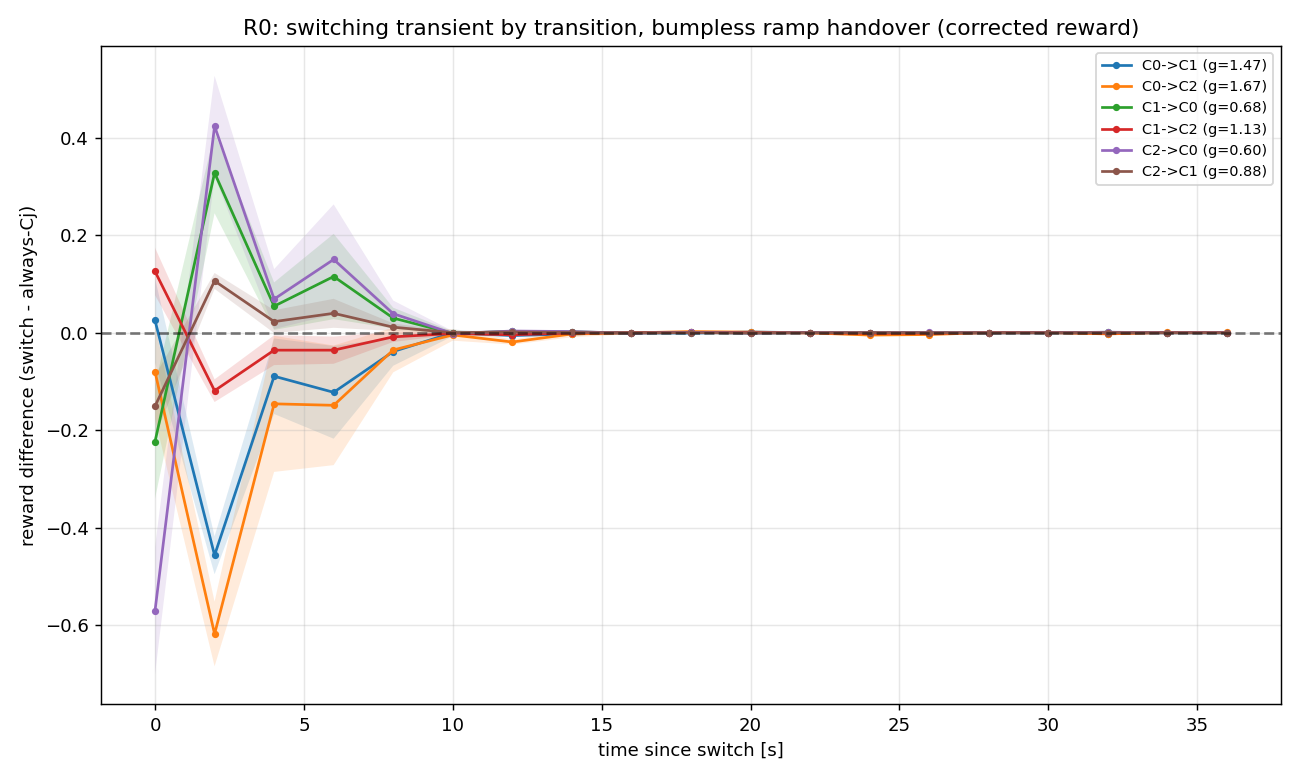
\includegraphics[width=0.78\linewidth]{figs/fig1_R0_transitions_ramp.png}
  \caption{Switching transient $\Delta r(t)$ in $R_0$ for all six transitions,
  with the realistic bumpless-ramp handover. The dip is shallow ($\lesssim 0.6$
  in reward) and recovers within a few seconds for every transition, so the
  switch cost is small under a proper handover.}
  \label{fig:transient}
\end{figure}

\subsection{Transient cost and its asymmetry}\label{sec:sw-cost}
A switch produces a brief reward dip; the loop remains stable throughout (no
divergence). With the \emph{naive} handovers the cost is strongly asymmetric in
the direction of the gain change: gain-\emph{decreasing} switches (from a higher-
to a lower-gain controller) are far costlier than gain-increasing ones, the
extreme case in $R_0$ being $\Ct\!\to\!\Cz$ (the largest gain drop), which
reflects the abrupt re-equilibration of the loop when the effective gain changes
discontinuously. With the realistic handovers this asymmetry is largely removed
(Fig.~\ref{fig:transient}): every transition incurs only a shallow, few-second
dip.

\subsection{Dependence on the handover implementation}\label{sec:sw-handover}
The magnitude of the transient depends far more on \emph{how} the controller is
handed over than on the transition itself. We compare four implementations of
the switch:
\begin{itemize}
  \item \textbf{naive carry-over (``hot'')}: the outgoing controller's internal
  filter state is transferred verbatim into the incoming controller. Because the
  gain difference resides in an internal filter section, the carried state is
  mis-scaled and the transient is \emph{worsened}.
  \item \textbf{state reset (``cold'')}: the incoming controller's filter state
  is zeroed. In a digital control system this produces an output discontinuity
  and an actuator impulse, and is not representative of switching a loop that
  must remain locked.
  \item \textbf{parallel banks}: all candidate controllers run continuously on
  the same error, each maintaining its own state; only the active output drives
  the suspensions. A switch changes which output is applied, producing a clean
  $(g_j/g_i)$ step in actuation.
  \item \textbf{bumpless ramp}: as parallel banks, but the applied command is
  cross-faded between the outgoing and incoming controller outputs over a short
  window, $u(t) = (1-\alpha)\,u^{(i)}(t) + \alpha\,u^{(j)}(t)$ with $\alpha:
  0\!\to\!1$. For this gain family the blend is exactly a continuous slew of the
  effective loop gain from $g_i$ to $g_j$, and is stable provided the loop has
  gain margin across the range. This models the gain-ramped, parallel-filter-bank
  handover used in detector digital-control systems.
\end{itemize}
Table~\ref{tab:handover} and Fig.~\ref{fig:handover} compare these on the worst
relevant case, $\Ct\!\to\!\Cz$ (a switch into the $R_0$ optimum). The integrated
loss spans more than two orders of magnitude: the naive carry-over is by far the
worst, state reset and parallel banks are comparable and moderate, and a short
($\sim$\,\SI{2}{s}) bumpless ramp very nearly eliminates the transient.

\begin{table}[t]
  \centering
  \caption{Switching cost for $\Ct\!\to\!\Cz$ in $R_0$ (gain ratio $0.60$) by
  handover implementation. Integrated loss in (raw score)$\cdot$\si{s}; dip in
  raw score.}
  \label{tab:handover}
  \begin{tabular}{lccl}
    \toprule
    Handover & integrated loss & dip depth & realism \\
    \midrule
    naive carry-over (hot)    & $-140$  & $-20.3$ & implementation artifact \\
    state reset (cold)        & $-8.4$  & $-3.3$  & actuator impulse; unrealistic in lock \\
    parallel banks            & $-5.1$  & $-2.2$  & realistic; gain-step \\
    bumpless ramp, \SI{8}{s}  & $-2.8$  & $-1.1$  & realistic; smooth \\
    bumpless ramp, \SI{2}{s}  & $\mathbf{+0.2}$ & $\mathbf{-0.6}$ & realistic; near-eliminated \\
    \bottomrule
  \end{tabular}
\end{table}

\begin{figure}[t]
  \centering
  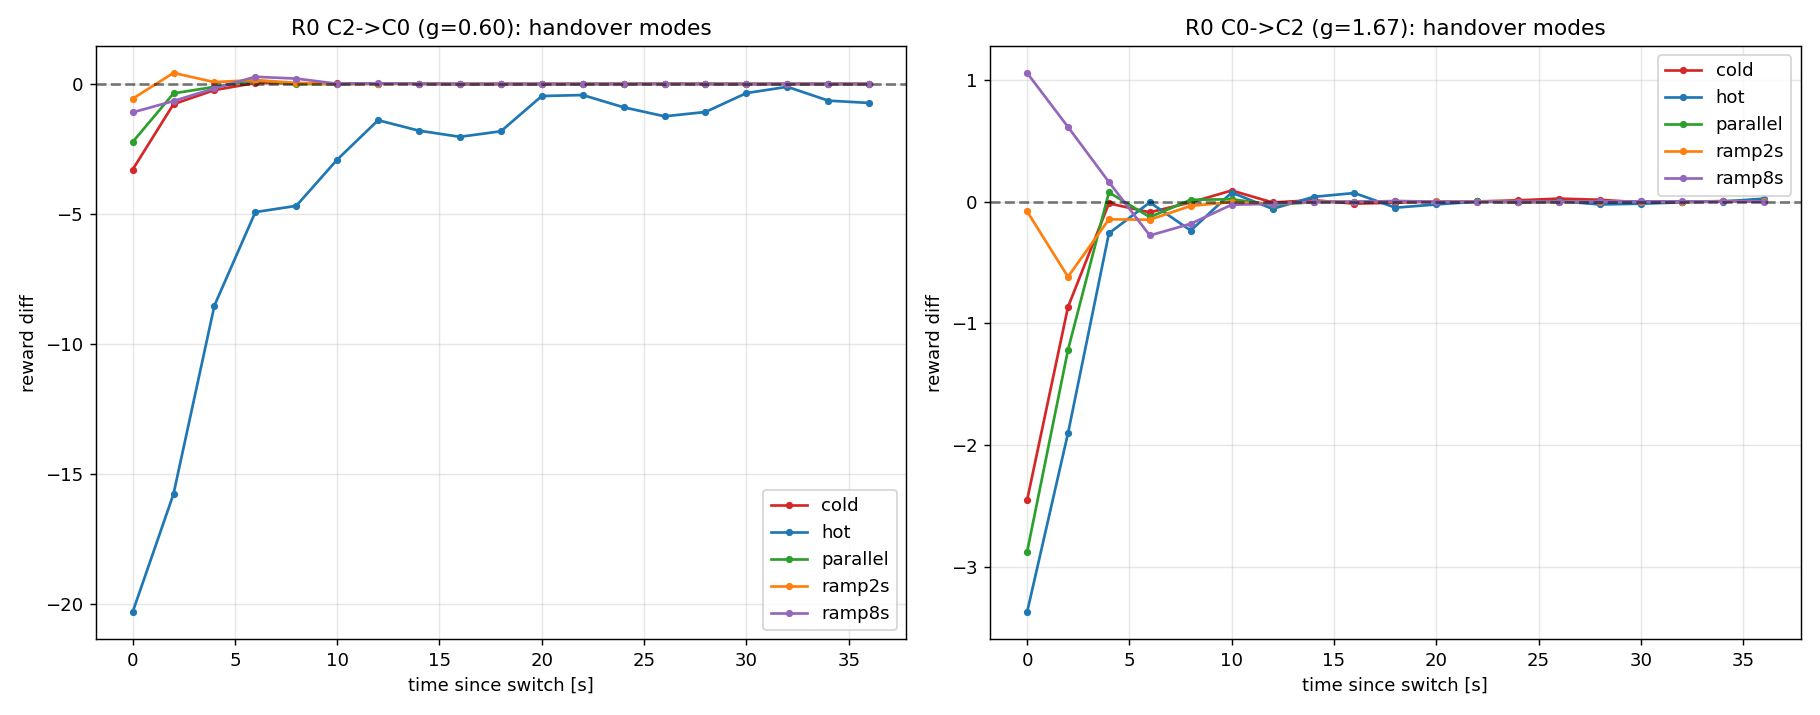
\includegraphics[width=0.92\linewidth]{figs/fig6_handover_modes.png}
  \caption{Switching transient by handover implementation, for
  $\Ct\!\to\!\Cz$ (left) and $\Cz\!\to\!\Ct$ (right) in $R_0$. A bumpless ramp
  (orange/purple) suppresses the transient that the naive carry-over (blue) and,
  to a lesser extent, the state reset (red) and parallel-bank (green) handovers
  exhibit.}
  \label{fig:handover}
\end{figure}

The central conclusion is that the apparent switching penalty is, for this
controller family, largely an artifact of the handover \emph{implementation}
rather than an intrinsic physical cost. With a bumpless, parallel-bank handover
the per-switch transient (integrated loss $\lesssim 1$ in reward$\cdot$s; a
few-second dip of $\lesssim 0.6$) is small: averaged over a hold window of
hundreds of seconds it shifts the window-mean reward by far less than the
per-regime separation between controllers (Section~\ref{sec:reward}), so an
online policy can switch freely. Two qualifications apply. First, this relies on the
controllers forming a gain family, for which the cross-fade is provably a smooth
gain slew; for controllers of different shape---e.g.\ future learned
controllers---a convex blend of two stabilising controllers is not guaranteed to
be stabilising mid-ramp, and the switching cost must be re-measured. Second, even
an ideal handover cannot remove the physical re-equilibration of the loop to a
different closed-loop bandwidth; the recovery times of a few seconds reflect this
irreducible component.

% =====================================================================
\section{Online controller selection}\label{sec:bandit}
% ---------------------------------------------------------------------

\subsection{The decision problem and its difficulties}\label{sec:ba-problem}
The policy observes, once per decision window of $T_{\mathrm{hold}}=\SI{100}{s}$,
a single number: the window-mean reward of the controller it chose to play. It
observes \emph{nothing else}---no regime label, no seismometer channel, no
forecast. (Only the reference Oracle is given the true regime mixture.) On this
information it must repeatedly choose the next controller. The
characterisation of Sections~\ref{sec:reward}--\ref{sec:switch} makes the
problem concrete, and hard, in five specific ways.

\begin{enumerate}
  \item \textbf{Partial observability of the regime.} The regime identity is
  carried by the \emph{shape} of the per-arm mean-reward vector
  (Fig.~\ref{fig:reward}), but a policy playing one arm per window sees one
  coordinate of that vector at a time. Worse, the achievable reward
  \emph{levels} of $R_0$ and $R_2$ nearly coincide, so a change $R_0
  \!\leftrightarrow\! R_2$ can be invisible in the reward stream of the
  currently played arm: detecting it may require playing arms that are
  currently believed suboptimal.
  \item \textbf{Noise-to-gap ratio.} The per-window reward noise
  ($\hat\sigma \approx 0.041$) exceeds the $R_1$ arm gap ($0.013$) and dwarfs
  the $R_2$ gap ($0.005$). Identification therefore costs many windows, and an
  algorithm that re-identifies from scratch at every regime visit pays this
  cost at every visit.
  \item \textbf{Recurrence.} The environment revisits the same three regimes
  (Section~\ref{sec:bg-env}) hundreds of times over months. This is the
  structure a good policy must exploit: knowledge accumulated in past visits
  of a regime remains valid and should be \emph{resumed}, not re-learned.
  \item \textbf{Continuous transitions.} Regime changes are ramps, not jumps
  (the adiabatic principle of Section~\ref{sec:bg-env}). During deep
  transitions the reward of \emph{every} arm collapses transiently; a
  change detector tuned only for level drops can mistake the collapsed,
  uniformly flat reward landscape for a new stationary regime and corrupt its
  statistics---a failure mode we repeatedly observed in earlier design
  iterations of the policy.
  \item \textbf{Short episodes.} $R_1$ storms last tens of minutes: an
  identification procedure whose budget exceeds the episode length never
  learns that regime at all, no matter how statistically sound it is.
\end{enumerate}

Two facts work in the policy's favour. Switching is nearly free under the
bumpless handover (Section~\ref{sec:switch}), so exploration is cheap at the
actuation level; and the number of distinct regimes is small, so a memory of
per-regime statistics is compact. The design question is therefore not
``how to forget the past'' (the premise of discounted methods) but ``how to
\emph{file} the past under the right regime and retrieve it on recurrence.''

\subsection{Policies compared}\label{sec:ba-algos}
We benchmark three groups of policies, all consuming the identical reward
stream defined above.

\paragraph{References.} Each \textbf{fixed controller} $\Cz,\Co,\Ct$; an
\textbf{Oracle} that is given the true regime mixture at each decision and
plays the argmax of the calibrated reward table (upper bound); and a
\textbf{rule-based} policy modelling current operator practice: an
exponentially weighted moving average of the observed reward triggers an alarm
when it stays below a calibrated floor, a routine re-check fires periodically
regardless, and either trigger starts a short round-robin probe of all
controllers, committing to the best measured. By construction this baseline is
blind to level-preserving regime changes (difficulty~1) except through its
periodic re-check.

\paragraph{Passively forgetting bandits.} Discounted UCB~\cite{GarivierMoulines}
and discounted (Gaussian) Thompson sampling~\cite{Thompson,RussoTutorial}, both
with discount $\gamma = 0.999$; a sweep over $\gamma$ did not qualitatively
change their behaviour. These treat non-stationarity as generic drift and
carry no regime memory.

\paragraph{The proposed policy.} Recurrence-Aware Thompson Sampling
(Section~\ref{sec:ba-rats}), together with three ablations that isolate its
design choices.

\subsection{Recurrence-Aware Thompson Sampling (RA-TS-F)}\label{sec:ba-rats}
RA-TS-F is a deliberately minimal answer to the difficulty list of
Section~\ref{sec:ba-problem}: \emph{just} Thompson sampling, a drift detector,
and a library of per-regime posteriors, arranged so that regime identification
\emph{emerges} from Thompson sampling's own exploration---with no scheduled
probing, no separate identification phase, and no statistical certification
step. (We arrived at it by successively removing exactly such machinery from
earlier design iterations, each removal improving both simplicity and regret.)
It has two internal modes.

\paragraph{TRACK.} The policy believes the environment is in a known regime
$g$ and runs standard Gaussian Thompson sampling on that regime's
\emph{accumulated} posterior: for each arm $a$, with $n_{g,a}$ past rewards
summing to $s_{g,a}$, the posterior over the mean reward is the conjugate
\begin{equation}
  \mu_{g,a} \,\big|\, \mathcal D \;\sim\; \mathcal N\!\left(
  \frac{\mu_0/\tau_0^2 + s_{g,a}/\hat\sigma^2}{1/\tau_0^2 + n_{g,a}/\hat\sigma^2},
  \;\Big(1/\tau_0^2 + n_{g,a}/\hat\sigma^2\Big)^{-1}\right),
  \label{eq:posterior}
\end{equation}
and the played arm is the argmax of one sample per arm. Exploitation
therefore becomes near-deterministic as evidence accumulates---\emph{without}
any explicit commit step---while a persistent small exploration probability
remains wherever arms are genuinely close (as in $R_2$), which is exactly
where exploration stays cheap. Each observed reward also feeds a per-arm
CUSUM~\cite{Page} drift statistic
\begin{equation}
  G_a \leftarrow \max\!\big(0,\; G_a + |r - b_a| - \nu\big), \qquad
  \text{alarm when } G_a \ge h,
  \label{eq:cusum}
\end{equation}
where $b$ is a \emph{frozen snapshot} of the regime's per-arm means taken when
the regime was adopted (so the detector cannot blind itself by tracking the
drift it is meant to detect), $\nu = 1.3\,\hat\sigma$ is a slack absorbing
noise, and $h = 8\,\hat\sigma$ sets the detection-delay/false-alarm trade-off.
An alarm empties the working state and enters ACQUIRE; the library entry keeps
its evidence.

\paragraph{ACQUIRE.} After an alarm (or at start-up) the working posterior is
reset to a diffuse prior ($\tau_0 = 0.5$), so Thompson sampling naturally
rotates across arms. A \emph{bounded coverage floor}---the ``-F'' in
RA-TS-F---plays the least-sampled arm whenever some arm has fewer than
$n_{\min}=3$ samples; this is the entire forced-exploration budget, at most
$n_{\min}K = 9$ windows per re-acquisition. Once covered, the centred shape of
the acquisition estimate, $\psi = \hat\mu - \overline{\hat\mu}$, is compared
with the centred shape of every library regime; centring cancels any common
reward level, making recognition level-invariant by construction
(difficulty~1). The nearest regime is \emph{resumed}---its posterior restored
and the acquisition samples folded in---only if it matches within a tolerance
($0.8\,\Delta_{\mathrm{sh}}$, with $\Delta_{\mathrm{sh}} \approx 0.053$ the
calibrated minimum shape separation between regimes) \emph{and} beats the
runner-up by a margin ($0.4\,\Delta_{\mathrm{sh}}$); a shape separated from
every known regime, once matured ($n_{\mathrm{new}}=8$ samples per arm),
founds a new library entry. There is no scheduled probe, no certification
test, no explicit level estimate, and no assumed number of regimes.

Why this works here can be read off the difficulty list: recurrence is
exploited by resuming posteriors, so the noise-to-gap cost (difficulty~2) is
paid once per regime rather than once per visit; level-invariant shape matching
handles the level-degenerate $R_0/R_2$ pair; the coverage floor guarantees the
few loser-arm samples that identification needs; and because acquisition is
Thompson sampling itself, the exploration performed while identifying is
simultaneously near-optimal exploitation---identification is not a separate
tax. The floor is not optional: plain RA-TS (identical but with the floor disabled)
\emph{stalls}, because Thompson sampling's very purpose is to stop playing
losing arms, so arm coverage is never reached, identification never completes,
and the policy degenerates to nearly-fixed play (85--129 switches per week
against RA-TS-F's $\sim$\,850; regret $3.6$--$5.9\times$ worse,
Table~\ref{tab:week}).

Fig.~\ref{fig:ratsdemo} shows the mechanism in the cleanest possible setting:
an instrumented \emph{toy} environment with synthetic rewards drawn from three
recurring regimes that switch \emph{discretely} (abrupt boundaries, equal
reward levels, a single fixed gap), using the same detector and matching
calibration as the production runs. The CUSUM statistic of the played arm rests
near zero within a regime, rises sharply at each hidden switch, and every alarm
is followed by a brief ACQUIRE probe (shaded, a few steps each) after which the
correct regime is recognised and its posterior resumed. Crucially, because the
regimes here are clean and discrete, the library settles at exactly $J=3$---one
entry per true regime---and the tracked regime $g(t)$ matches the truth $z(t)$
throughout.

This is deliberately \emph{not} what happens in the physical environment, and
the difference is instructive. In the detector simulations the library grows
beyond the three nominal regimes ($J=8$ over one week, $J=17$ over six months;
Figs.~\ref{fig:weekinternals} and Sec.~\ref{sec:ba-sixmo}) for two reasons
absent from the toy. First, the regime gaps are tiny and unequal (down to
$0.005$ in $R_2$) and identification runs on only $n_{\min}\!=\!3$ noisy probe
samples per arm, so a recurring regime whose noisy shape estimate misses its
match margin occasionally founds a duplicate entry rather than resuming the
original. Second, and more fundamentally, the physical regime transitions are
\emph{continuous ramps}, not the toy's instantaneous switches
(Section~\ref{sec:bg-env}); the mid-ramp blended states are genuinely distinct
reward shapes and the algorithm faithfully files them as short-lived extra
entries (Sec.~\ref{sec:ba-sixmo} quantifies this). Neither effect degrades
performance---duplicate entries converge to the same best arm and transition
entries cover genuinely ambiguous windows---which is why RA-TS-F attains the
lowest regret despite carrying a ``dirtier'' library than the toy's clean
$J=3$. The toy thus isolates the mechanism; the real runs show it remains
effective when the discrete-regime idealisation is only approximate.

\begin{figure}[t]
  \centering
  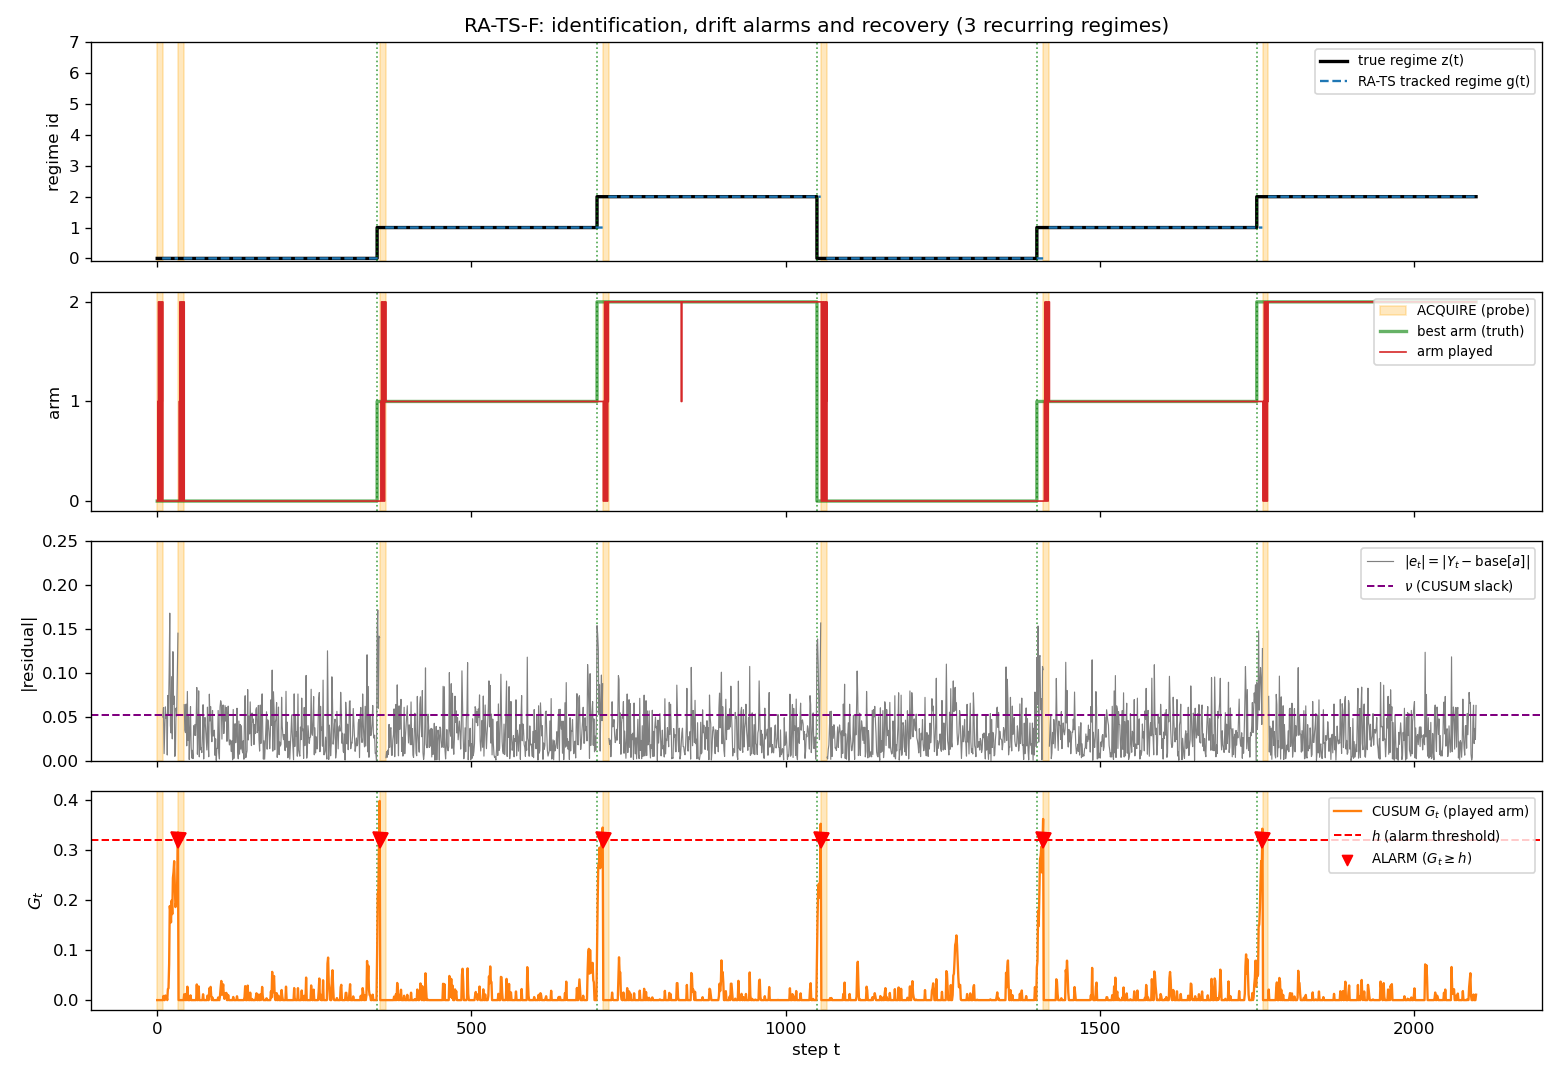
\includegraphics[width=\linewidth]{figs/rats_overview.png}
  \caption{RA-TS-F mechanics on a \emph{clean toy} environment: synthetic
  rewards, three recurring regimes with discrete switches and equal reward
  levels, same detector/matching calibration as the production runs. From top:
  true regime $z(t)$ and tracked regime $g(t)$ (they coincide, and the library
  settles at exactly $J=3$); played arm vs.\ true best arm, with ACQUIRE probes
  shaded; per-step detector residual $|r - b_a|$ against the CUSUM slack $\nu$;
  CUSUM statistic $G$ with threshold $h$ and alarms. Every hidden switch drives
  $G$ over threshold within a few decisions; the subsequent ACQUIRE probe lasts
  only a handful of windows before the returning regime is recognised (shape
  match) and its posterior resumed. On the physical environment the same
  mechanism runs but the library grows beyond $J=3$ (tiny unequal gaps and
  continuous transitions; see text), without loss of regret.}
  \label{fig:ratsdemo}
\end{figure}

\subsection{Experimental protocol}\label{sec:ba-protocol}
All policies are run on \emph{identical}, pre-generated noise realisations
(common random numbers): the regime schedule, injected suspension noise, input
power, and per-window sensing noise are shared sample-by-sample, so policies
differ only through their choices, and cumulative-reward differences are
paired. The controller is held fixed within each $T_{\mathrm{hold}}=\SI{100}{s}$
window; switching uses the \SI{2}{s} bumpless handover; the reward filters run
continuously across the whole horizon (Section~\ref{sec:reward}). We use three
benchmarks: two one-week environments differing in storm frequency
(\emph{r1long}: one $R_1$ event per day on average; \emph{r1freq}: two per
day---roughly twice the regime switches), and one six-month environment
($1.55\times10^7$\,s, $\sim$\,$1.6\times10^5$ decisions, $181$ storm events and
$\sim$\,$3600$ diurnal drift transitions). The figure of merit is cumulative
regret against the Oracle; we also report the total number of controller
switches and the fraction of windows in which a \emph{near-optimal} controller
is played. We call a controller near-optimal in a window when its expected
per-window reward is within $\varepsilon = \tfrac12\hat\sigma \approx 0.021$ of
the best achievable (with $\hat\sigma$ the calibrated per-window reward noise).
This is a more informative accuracy metric than the strict optimal-arm rate
because two controllers are genuinely near-tied in some regimes---most sharply
$\Co$ and $\Ct$ in $R_2$, gap $0.005$ (Table~\ref{tab:reward})---so playing the
runner-up there costs essentially no regret; $\varepsilon$ sits an order of
magnitude below every \emph{costly} confusion (gaps $\ge 0.08$), so the metric
counts only genuine mistakes and, unlike the strict rate, tracks regret rather
than contradicting it.

\subsection{Results: one-week benchmarks}\label{sec:ba-results}

\begin{table}[t]
  \centering
  \caption{One-week benchmarks: cumulative regret vs.\ the Oracle (lower is
  better) and number of controller switches, on the identical noise realisation
  per column. $\sim$\,$6000$ decisions per run. Oracle cumulative reward:
  $2153.9$ (r1long), $2138.6$ (r1freq).}
  \label{tab:week}
  \begin{tabular}{l cc c cc}
    \toprule
     & \multicolumn{2}{c}{regret} & & \multicolumn{2}{c}{switches} \\
     \cmidrule(lr){2-3}\cmidrule(lr){5-6}
    policy & r1long & r1freq & & r1long & r1freq \\
    \midrule
    \textbf{RA-TS-F}            & $\mathbf{40.7}$ & $\mathbf{25.8}$ & & 896  & 820 \\
    RA-TS-FR (rollback)         & 40.6  & 37.8  & & 959  & 1188 \\
    RA-TS-FQ (delayed commit)   & 41.1  & 39.3  & & 1058 & 1020 \\
    RA-TS (no coverage floor)   & 147.0 & 152.2 & & 85   & 129 \\
    \midrule
    Rule-based                  & 125.1 & 175.6 & & 68   & 64  \\
    D-UCB                       & 159.6 & 154.1 & & 1985 & 2047 \\
    Thompson (discounted)       & 176.8 & 170.6 & & 33   & 31  \\
    \midrule
    Fixed-$\Cz$                 & 155.9 & 151.2 & & 0 & 0 \\
    Fixed-$\Co$                 & 191.0 & 188.7 & & 0 & 0 \\
    Fixed-$\Ct$                 & 217.2 & 216.1 & & 0 & 0 \\
    \bottomrule
  \end{tabular}
\end{table}

\begin{figure}[t]
  \centering
  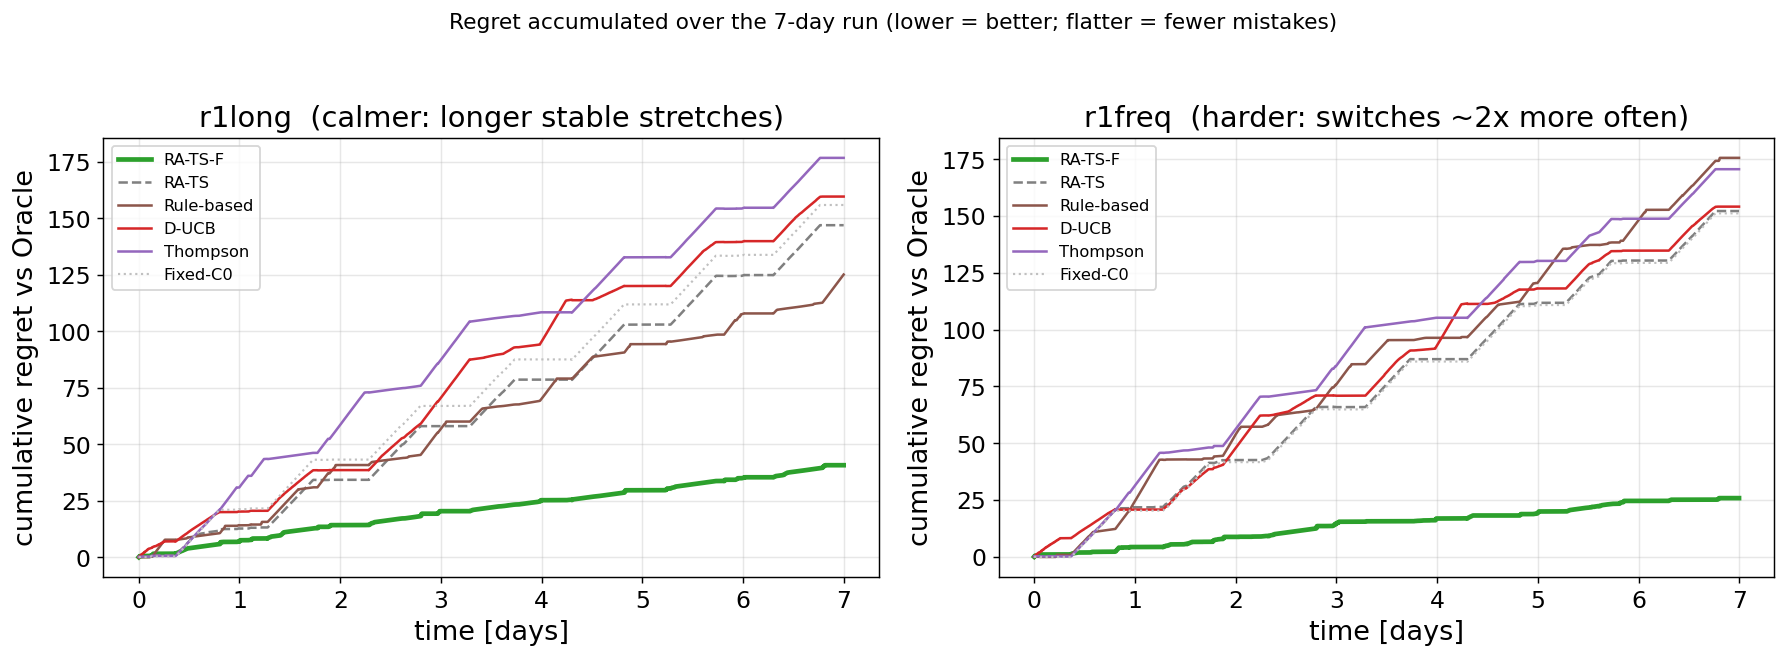
\includegraphics[width=0.98\linewidth]{figs/week_regret_curves.png}
  \caption{Cumulative regret against the Oracle over the two one-week
  benchmarks. RA-TS-F (green) accumulates regret at a rate $3$--$6\times$ lower
  than every baseline, and its advantage widens on the harder cache (right).
  RA-TS without the coverage floor (grey dashed) stalls and tracks the
  fixed-controller slope (dotted), its stepped growth marking mis-handled
  regime episodes; the discounted bandits (red, purple) barely improve on the
  best fixed controller; the rule-based policy (brown) is competitive on the
  calm cache but degrades under frequent switching.}
  \label{fig:weekregret}
\end{figure}

RA-TS-F attains by far the lowest regret on both caches (Table~\ref{tab:week},
Fig.~\ref{fig:weekregret}): $40.7$ on r1long and $25.8$ on r1freq, against
$125$--$217$ for every baseline. Two features of this gap deserve emphasis.
First---important for robustness---RA-TS-F's advantage \emph{grows} on the
harder, more frequently switching cache, where every baseline stagnates or
degrades. This is the recurrence dividend: a policy without regime memory
re-pays the identification cost at every regime episode, so doubling the
episode rate doubles that loss, while RA-TS-F's per-episode cost is a few
probe windows followed by a posterior resume. Second, the failure modes of the
baselines are exactly the difficulties of Section~\ref{sec:ba-problem}: the
rule-based operator policy degrades sharply with switching frequency
($125 \to 176$), the price of level-blind, schedule-driven re-checking
(difficulty~1); and the passively forgetting bandits are barely better than
the best fixed arm on either cache---generic forgetting cannot exploit
recurrence (difficulty~3), and by continually discarding evidence it never
resolves the small gaps (difficulty~2). Measured against the best fixed
controller ($\Cz$, regret $155.9$/$151.2$), RA-TS-F captures $74\%$/$83\%$ of
the achievable Oracle advantage.

The two purity-preserving ablations of RA-TS-F probe whether library
contamination---post-switch samples committed to the old regime during the
detection delay---matters in practice. Rollback (FR) retroactively un-commits
the change-point run on each alarm; delayed commit (FQ) quarantines samples for
$q=10$ rounds. Neither helps: both match RA-TS-F on r1long and lose on r1freq
(where FQ's stale posterior and FR's discarded evidence cost most), so the
plain tolerance-based design is not merely simpler but empirically the best of
the three.

\begin{figure}[t]
  \centering
  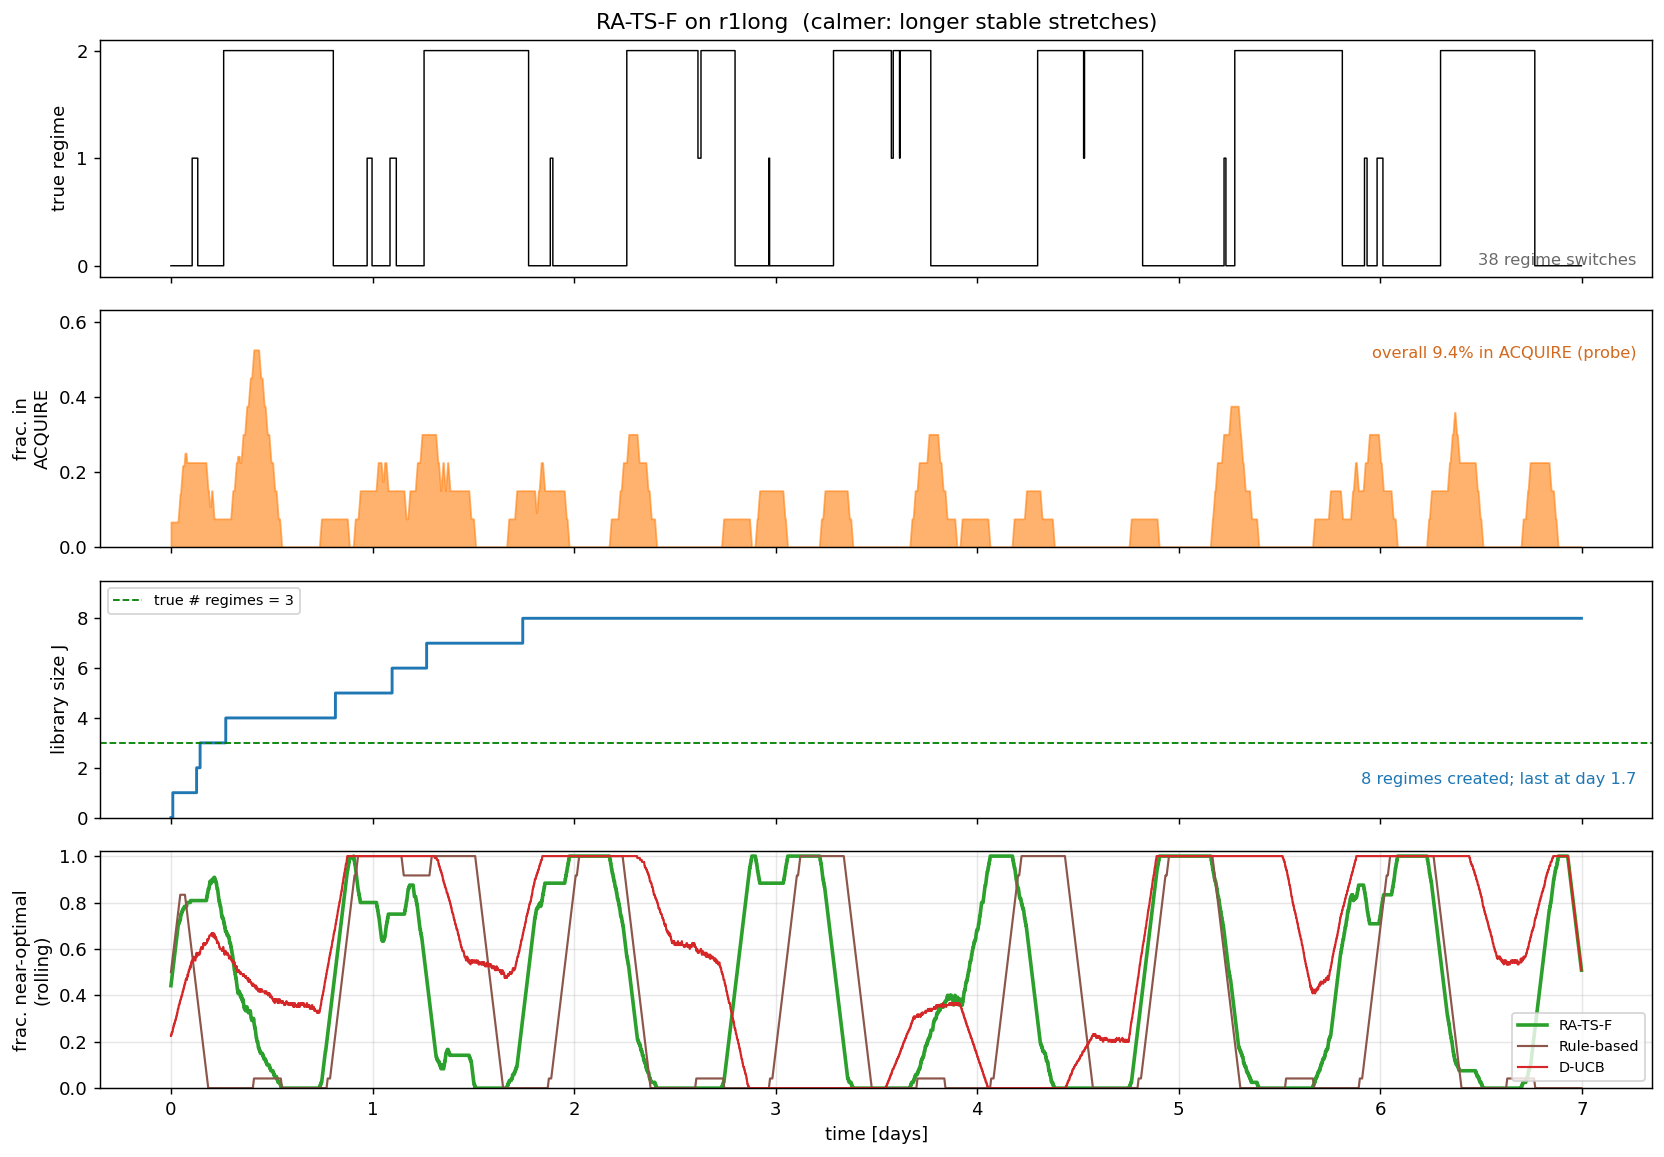
\includegraphics[width=0.98\linewidth]{figs/week_internals_r1long.png}
  \caption{RA-TS-F internals over the r1long week (three stacked panels). From
  top: (i) the true regime sequence ($38$ switches); (ii) the fraction of
  decisions spent in ACQUIRE (the re-identification probe), shown as a rolling
  average over a $\SI{3.3}{h}$ ($120$-decision) sliding window---probing is
  $9.4\%$ of decisions overall and occurs in short bursts localised at the
  regime boundaries, so between boundaries the policy is pure warm-posterior
  exploitation; (iii) the library size $J$, which stabilises by day $1.7$ at
  $J=8$ (the three true regimes plus noise-split duplicates, see text) and adds
  no further entries over the remaining five days.}
  \label{fig:weekinternals}
\end{figure}

Fig.~\ref{fig:weekinternals} dissects \emph{how} RA-TS-F spends its budget on
r1long. Probing (ACQUIRE) accounts for $9.4\%$ of decisions and is concentrated
in short bursts at the regime boundaries---between alarms the policy is pure
warm-posterior exploitation. The library stabilises within two days and no new
entries are created for the remaining five. Its final size is $J=8$ rather
than $3$: with $n_{\min}=3$ probe samples per arm, the shape-estimate noise is
comparable to the small calibrated separation $\Delta_{\mathrm{sh}}$, so a
recurring regime occasionally fails its match margin and founds a duplicate
entry. Duplicates are benign---each converges to the same best arm, and the
regret cost of maturing one is a few windows---but they mark the price of
identifying from only $n_{\min}K$ noisy samples; we return to this at the
six-month scale.

\subsection{Results: six-month run}\label{sec:ba-sixmo}

\begin{table}[t]
  \centering
  \caption{Six-month run ($180$ days, $155{,}519$ decisions, identical noise
  realisation for all policies): cumulative regret vs.\ the Oracle, fraction of
  windows playing a near-optimal controller (within $\tfrac12\hat\sigma$ of the
  best, Section~\ref{sec:ba-protocol}), and number of switches. Oracle
  cumulative reward $57106.4$.}
  \label{tab:sixmo}
  \begin{tabular}{l r r r}
    \toprule
    policy & regret & frac.\ near-opt. & switches \\
    \midrule
    Oracle             & $0$      & $0.997$ & $865$ \\
    \textbf{RA-TS-F}   & $\mathbf{861.5}$ & $0.936$ & $16{,}959$ \\
    Rule-based         & $3702.9$ & $0.626$ & $1683$ \\
    Fixed-$\Cz$        & $3872.7$ & $0.508$ & $0$ \\
    Thompson (disc.)   & $4095.3$ & $0.509$ & $437$ \\
    Fixed-$\Co$        & $5235.0$ & $0.522$ & $0$ \\
    D-UCB              & $5319.3$ & $0.521$ & $44{,}255$ \\
    Fixed-$\Ct$        & $6005.2$ & $0.501$ & $0$ \\
    \bottomrule
  \end{tabular}
\end{table}

\begin{figure}[t]
  \centering
  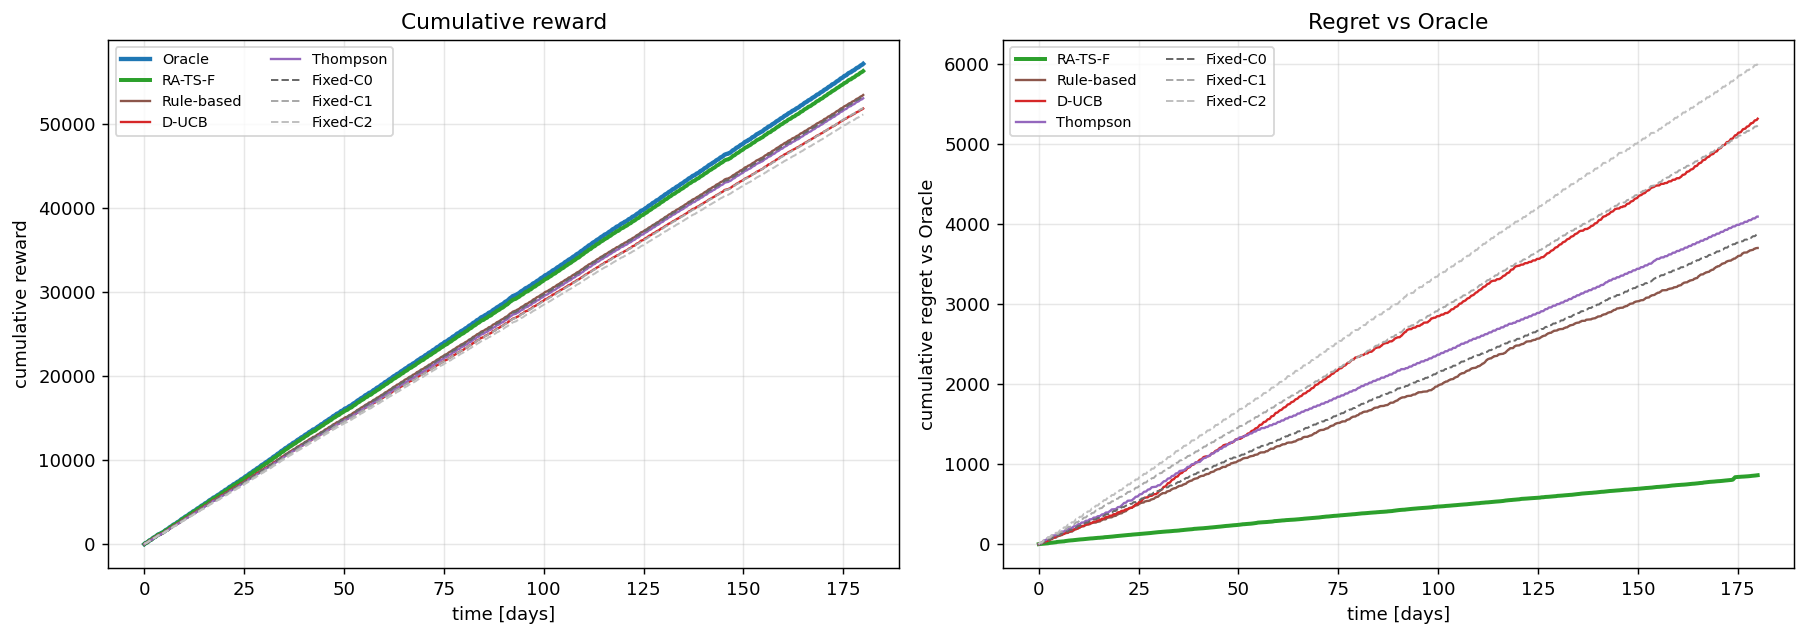
\includegraphics[width=0.98\linewidth]{figs/sixmo_cumreward_regret.png}
  \caption{Six-month run: cumulative reward (left) and cumulative regret
  against the Oracle (right) for all policies. RA-TS-F's regret grows at a
  near-constant, far shallower slope than every alternative throughout the
  $180$ days---there is no late-horizon degradation, saturation of the
  advantage, or drift-induced breakdown.}
  \label{fig:sixmo}
\end{figure}

\begin{figure}[t]
  \centering
  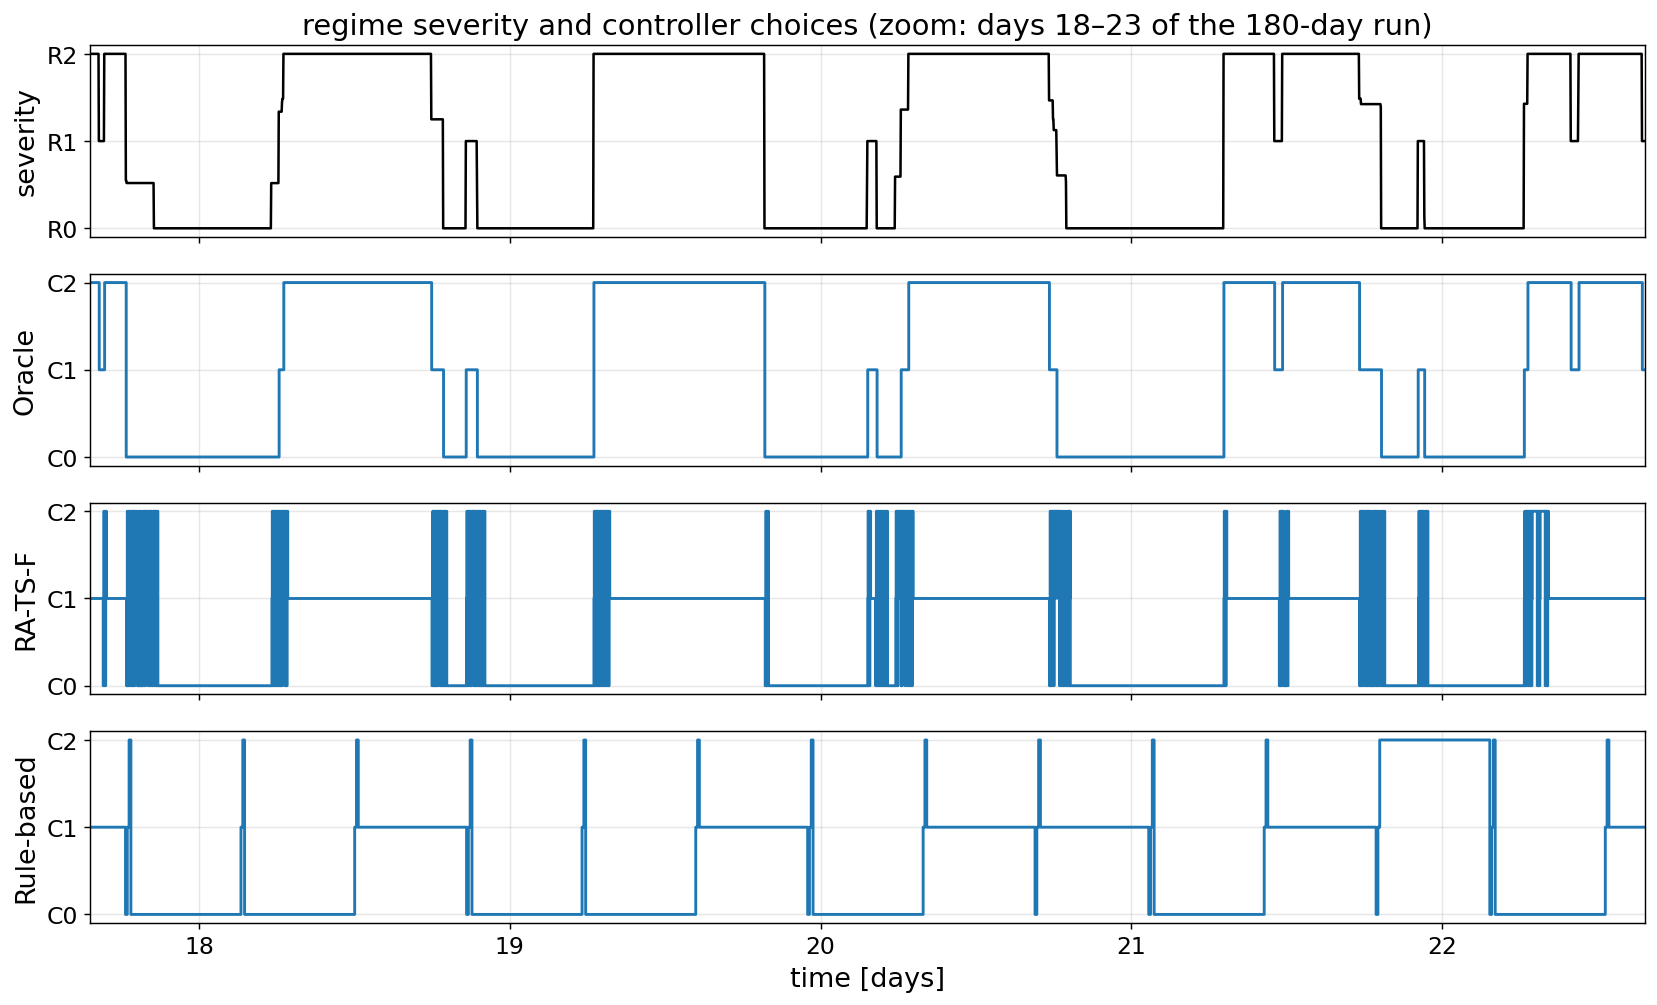
\includegraphics[width=0.98\linewidth]{figs/sixmo_timelines.png}
  \caption{Six-month run, zoomed to a representative $5$-day window (the full
  $180$-day timeline is an unreadable dense band). Top: regime severity
  ($R_0/R_1/R_2$). Below: controller choices of the Oracle, RA-TS-F, and the
  rule-based policy. RA-TS-F tracks the regime structure closely---it plays
  $\Cz$ through the $R_0$ stretches and captures the $R_1$ spikes, with brief
  vertical bursts marking the acquisition probes at each boundary. Through the
  $R_2$ stretches it settles on $\Co$ rather than the Oracle's $\Ct$: the two
  are near-tied there (gap $0.005$, Fig.~\ref{fig:reward}), so Thompson sampling
  does not distinguish them and the choice costs essentially no regret---this is
  precisely why the near-optimal fraction, not the strict optimal-arm rate, is
  the meaningful accuracy metric (Table~\ref{tab:sixmo}). The rule-based policy
  switches rarely ($1683$ total) and visibly lags the severity pattern, its
  re-checks being schedule- rather than event-driven.}
  \label{fig:sixmotimelines}
\end{figure}

The six-month run tests whether the one-week picture survives scale, slow
parameter drift, and hundreds of regime episodes. It does
(Table~\ref{tab:sixmo}, Figs.~\ref{fig:sixmo}--\ref{fig:sixmotimelines}):
RA-TS-F's regret of $861.5$ is $4.3\times$ lower than the best alternative
(the rule-based policy) and up to $7\times$ lower than the rest, capturing
$78\%$ of the Oracle's advantage over the best fixed controller---%
quantitatively consistent with the one-week ratios, i.e.\ the advantage is not
a short-horizon artefact. The mean per-window regret is $0.0055 \approx
0.13\,\hat\sigma$. The switch counts show that switching a lot is neither
necessary nor sufficient: D-UCB switches $44$k times for the worst learner
regret, the rule-based policy only $1683$ times, and RA-TS-F sits between
($17$k, $11\%$ of decisions) with its exploration event-triggered by the
drift detector rather than scheduled. The near-optimal fraction sharpens the
picture: RA-TS-F plays a near-optimal controller in $93.6\%$ of all windows,
against $\le 63\%$ for every baseline and only $\sim 51\%$ for any fixed
controller. (The strict optimal-arm rate is misleading here---it scores
RA-TS-F at $0.48$, tying Fixed-$\Cz$, because $R_0$ dominates the duty cycle
and it gives no credit for playing the near-tied runner-up in $R_2$; the
near-optimal rate removes that artefact and cleanly separates the policies in
the same order as regret.) Notably each fixed controller is near-optimal in
almost exactly the fraction of time its regimes are active
($\sim 0.5$)---strong on its own regimes, wrong elsewhere---whereas RA-TS-F is
near-optimal almost everywhere, which is precisely the behaviour an
autonomous selector must provide.

Two further observations from the six-month diagnostics. First, the regret
slope of RA-TS-F is stable across the entire horizon
(Fig.~\ref{fig:sixmo}, right): the resumed posteriors do not go stale despite
the environment's slow within-regime drift ($\sim$\,$3600$ drift transitions),
because the CUSUM alarm simply triggers re-acquisition whenever a stored
baseline stops matching. Second, the library grows to $J=17$ entries over
$180$ days. Diagnosing them individually shows the excess is \emph{not}
primarily duplicate noise: six entries are duplicates of the $R_0$/$R_1$
clusters (the same $n_{\min}$-probe effect seen at week scale), but eight are
short-dwell entries that map onto genuine \emph{transition states}---windows in
which the environment is mid-ramp between regimes ($13.5\%$ of tracked time;
even the Oracle's reward drops from $0.40$ to $0.19$ there). The algorithm, built
for discrete recurring regimes, faithfully discovers that this environment's
switches are continuous ramps and files the ramp as extra regimes. This is a
bookkeeping artefact with no measurable regret cost, but it delineates cleanly
where the discrete-regime model of the environment ends.

% =====================================================================
\section{Discussion}\label{sec:discussion}
% ---------------------------------------------------------------------
The infrastructure and measurements above delimit what an online controller-
selection policy can and cannot achieve in this setting. The regime--controller
problem is well posed, with the one-to-one mapping holding in all three regimes
and a non-saturating reward; the per-regime separation is largest in the nominal
regime and smallest (though still favouring the designed controller) in the
extreme regime, so the achievable advantage of a selection policy is modest and
accrues across all regimes. At the same time, with a realistic bumpless handover the cost of
switching is small, so regret is governed primarily by \emph{which} controller is
chosen rather than by the act of switching. These two observations frame the
bandit comparison of Section~\ref{sec:bandit}: the relevant question is how
quickly and reliably a policy identifies the regime-optimal controller as the
environment drifts, with switching essentially free.

The bandit results answer that question with a clear structural message:
exploiting \emph{recurrence} is what matters. Resuming per-regime knowledge
beats re-learning it at every episode, and beats forgetting it (the discounted
baselines) by a wide margin. Just as telling is what proved unnecessary: our
earlier design iterations carried scheduled probes, explicit identification
phases, and statistical certification tests, each added to fix a real failure
mode; all of them became removable once identification was made emergent from
Thompson sampling itself, guarded only by a bounded coverage floor---and every
removal improved regret. The floor is the one non-negotiable ingredient:
without it, Thompson sampling's own efficiency starves the identification
signal and the policy stalls ($3.6$--$5.9\times$ worse regret,
Table~\ref{tab:week}). Its cost is bounded ($n_{\min}K$ windows per
re-acquisition, $9.4\%$ of decisions in practice). A practical corollary for
detector operations: the reward signal that suffices for all of this is
computable online from existing error and control channels; no auxiliary
environmental sensing is required, although incorporating such context (e.g.\
seismometer bands or earthquake early warning) as side information is a
natural extension.

For future learned (e.g.\ neural-network) controllers two elements must be
revisited: the reward separation between arms is expected to grow (learned
controllers specialise more aggressively than a gain family), which makes the
selection problem easier; but the near-free switching result of
Section~\ref{sec:switch} relies on the gain-family structure and must be
re-measured, since a convex blend of two stabilising controllers of different
shape is not guaranteed stabilising mid-ramp. The RA-TS-F layer itself is
agnostic to both changes.

% =====================================================================
\section{Conclusion}\label{sec:conclusion}
% ---------------------------------------------------------------------
We posed the operational practice of switching angular-control filters as an
online controller-selection problem and built the infrastructure to study it
rigorously: a validated time-domain plant, three physically motivated operating
regimes with a designed one-to-one regime--controller mapping, a calibrated
multi-band reward computed online from the loop's own signals, and a
common-random-numbers benchmark spanning one-week and six-month horizons. Three
findings stand out. First, the selection problem is well posed but genuinely
hard: the reward distributions of the candidate controllers overlap strongly,
two of the three regimes are separated by gaps below the per-window noise, and
the regime identity is carried by the cross-arm reward \emph{shape} rather than
its level. Second, the apparent cost of switching controllers is dominated by
the handover implementation; with a bumpless, parallel-bank handover---standard
practice in detector digital control---switching is nearly free, removing the
main physical objection to autonomous switching. Third, a deliberately minimal
policy, Recurrence-Aware Thompson Sampling with a bounded coverage floor
(RA-TS-F), outperforms every alternative tested---discounted bandits, an
operator-like rule, and all fixed controllers---achieving $74$--$83\%$ of the oracle's
achievable advantage over the best fixed controller, with a regret slope that
remains constant over $180$ simulated days. The combination of a cheap
handover, an online reward from existing channels, and a simple
recurrence-aware policy makes autonomous alignment-configuration selection a
realistic operational prospect; extending the same framework to learned
controllers on hardware-validated setups is the natural next step.

% =====================================================================
\section*{Acknowledgements}
\todo{funding and computing acknowledgements.}

% =====================================================================
\begin{thebibliography}{99}
\bibitem{aLIGO} J.~Aasi \emph{et al.} (LIGO Scientific Collaboration),
  \emph{Advanced LIGO}, Class.\ Quantum Grav.\ \textbf{32}, 074001 (2015).
\bibitem{aVirgo} F.~Acernese \emph{et al.} (Virgo Collaboration),
  \emph{Advanced Virgo: a second-generation interferometric gravitational wave
  detector}, Class.\ Quantum Grav.\ \textbf{32}, 024001 (2015).
\bibitem{SidlesSigg} J.~A.~Sidles and D.~Sigg,
  \emph{Optical torques in suspended Fabry--Perot interferometers},
  Phys.\ Lett.\ A \textbf{354}, 167 (2006).
\bibitem{Barsotti} L.~Barsotti, M.~Evans, and P.~Fritschel,
  \emph{Alignment sensing and control in advanced LIGO},
  Class.\ Quantum Grav.\ \textbf{27}, 084026 (2010).
\bibitem{Lattimore} T.~Lattimore and C.~Szepesv\'ari,
  \emph{Bandit Algorithms}, Cambridge University Press (2020).
\bibitem{GarivierMoulines} A.~Garivier and E.~Moulines,
  \emph{On upper-confidence bound policies for switching bandit problems},
  in \emph{Algorithmic Learning Theory} (2011), p.~174.
\bibitem{AdSwitch} P.~Auer, P.~Gajane, and R.~Ortner,
  \emph{Adaptively tracking the best bandit arm with an unknown number of
  distribution changes}, in \emph{Proc.\ COLT} (2019).
\bibitem{Thompson} W.~R.~Thompson,
  \emph{On the likelihood that one unknown probability exceeds another in view
  of the evidence of two samples}, Biometrika \textbf{25}, 285 (1933).
\bibitem{RussoTutorial} D.~Russo \emph{et al.},
  \emph{A tutorial on Thompson sampling},
  Found.\ Trends Mach.\ Learn.\ \textbf{11}, 1 (2018).
\bibitem{Page} E.~S.~Page,
  \emph{Continuous inspection schemes}, Biometrika \textbf{41}, 100 (1954).
\bibitem{Harms_internal} \todo{replace with a citable reference (or remove)
  for the adiabatic-non-stationarity argument.}
\end{thebibliography}

\end{document}
